\documentclass[handout]{beamer}
\usetheme{metropolis}

% -------------------------------------------------------------------
%   PAQUETES
% -------------------------------------------------------------------
\usepackage[spanish,activeacute]{babel}     % Soporte para español
\usepackage{amsmath, amssymb}              % Matemáticas esenciales
\usepackage{graphicx}                      % Inclusión de imágenes
\usepackage{multirow}                      % Tablas complejas
\usepackage[ruled,vlined,lined]{algorithm2e}% Algoritmos
\usepackage{fontspec}                      % Manejo de fuentes con XeLaTeX
\setsansfont{Lato}                         % Fuente Sans
\setmonofont{Inconsolata}                  % Fuente Monospace
\usepackage{hyperref}                      % Enlaces clicables
\hypersetup{
    colorlinks=true,
    linkcolor=blue,
    urlcolor=magenta
}

% -------------------------------------------------------------------
%   INFORMACIÓN DEL DOCUMENTO
% -------------------------------------------------------------------
\title{Procesamiento del Lenguaje Natural \\ \large Preguntas fundamentales sobre el Lenguaje}
\author[Jorge Ortiz Fuentes]{Jorge Ortiz Fuentes}
\date{\today}

% -------------------------------------------------------------------
%   METADATOS / CONFIGURACIONES
% -------------------------------------------------------------------
\setbeamercolor{normal text}{fg=black,bg=white}
\setbeamercolor{alerted text}{fg=red!80!black}
\setbeamercolor{example text}{fg=green!50!black}
\setbeamertemplate{navigation symbols}{}
\setbeamertemplate{caption}[numbered]
\setbeamertemplate{footline}{
  \begin{beamercolorbox}[wd=\paperwidth,ht=2.5ex,dp=1ex]{frametitle}
    \vspace{1pt}
    \hfill \insertframenumber/\inserttotalframenumber \hspace{3mm}
  \end{beamercolorbox}
}
\metroset{block=fill}
% -------------------------------------------------------------------

\begin{document}

% -------------------------------------------------------------------
%   PORTADA
% -------------------------------------------------------------------
\begin{frame}
  \titlepage
\end{frame}

% -------------------------------------------------------------------
%   ÍNDICE
% -------------------------------------------------------------------
% \begin{frame}{Contenido}
%   \tableofcontents
% \end{frame}

% -------------------------------------------------------------------
%   SECCIÓN: INTRODUCCIÓN
% -------------------------------------------------------------------
\section{Introducción}

% 1. Motivación inicial
\begin{frame}{¿Por qué es importante pensar el lenguaje?}
  \begin{itemize}
    \item Es nuestro objeto de procesamiento en el NLP
    \item Existen muchas preguntas no resueltas
    \item ¡Es muy interesante!
  \end{itemize}
\end{frame}


% -------------------------------------------------------------------
%   DIAPOSITIVA: Pregunta 1
% -------------------------------------------------------------------
\begin{frame}{Pregunta para reflexionar}
  \centering
  \LARGE ¿Por qué los chilenos hablamos como hablamos?
\end{frame}

% -------------------------------------------------------------------
%   DIAPOSITIVA: Pregunta 2
% -------------------------------------------------------------------
\begin{frame}{Pregunta para reflexionar}
  \centering
  \LARGE ¿Es válido el lenguaje inclusivo?
\end{frame}

% -------------------------------------------------------------------
%   DIAPOSITIVA: Pregunta 3
% -------------------------------------------------------------------
\begin{frame}{Pregunta para reflexionar}
  \centering
  \LARGE ¿De dónde viene el lenguaje?
\end{frame}

% -------------------------------------------------------------------
%   SECCIÓN: SAUSSURE Y LAS BASES DE LA LINGÜÍSTICA
% -------------------------------------------------------------------
\section{Saussure y las bases de la lingüística moderna}

% 3. Breve biografía de Saussure
\begin{frame}{Ferdinand de Saussure (1857-1913)}
  \begin{columns}
    \begin{column}{0.4\textwidth}
      \begin{center}
        \includegraphics[width=0.9\textwidth]{pics/saussure.png}\\
        \vspace{0.2cm}
      \end{center}
    \end{column}
    \begin{column}{0.6\textwidth}
      \begin{itemize}
        \item Lingüista suizo, considerado \textbf{el padre de la lingüística moderna}
        \item Su obra póstuma, \textit{Curso de Lingüística General} (1916), estableció fundamentos para el estudio del lenguaje
    \end{itemize}
      \vspace{5pt}
      \textbf{Principales aportes:}
      \begin{itemize}
        \item Fue el primero en pensar la lingüística como una \textbf{ciencia} y propuso preguntas fundamentales sobre la \textbf{naturaleza del lenguaje}
      \end{itemize}
    \end{column}
  \end{columns}
\end{frame}


% -------------------------------------------------------------------
%   SECCIÓN: INDIVIDUAL VS. SOCIAL
% -------------------------------------------------------------------
\section{¿Es el lenguaje individual o social?}

% 5. Problemática inicial
\begin{frame}{El lenguaje como fenómeno complejo}
    \begin{block}{Pregunta clave}
      ¿Dónde “reside” el lenguaje? ¿En el individuo (cerebro) o en la sociedad (cultura)?
    \end{block}
    
    \begin{itemize}
      \item El estudio del lenguaje abarca dos grandes ámbitos:
        \begin{itemize}
            \item \textbf{Individuo:} Se estudian los procesos mentales (psicolingüística), la función cerebral relacionada (neurolingüística) y los mecanismos de adquisición y desarrollo del lenguaje
            \item \textbf{Sociedad:} Se estudian las variaciones y usos del lenguaje en contextos sociales (sociolingüística), las prácticas culturales (antropología lingüística) y la construcción de significados en contexto (análisis del discurso)
        \end{itemize}
    \end{itemize}
  \end{frame}

  % 6. Lenguaje como fenómeno individual
% -------------------------------------------------------------------
%   DIAPOSITIVA: Introducción al problema: Lenguaje como fenómeno individual
% -------------------------------------------------------------------
\begin{frame}{Lenguaje como fenómeno individual: una introducción}
    \begin{columns}
        \begin{column}{0.65\textwidth}
          \begin{itemize}
            \item El lenguaje humano es posible gracias a la anatomía humana
            \item Aunque se conocen áreas clave (Broca, Wernicke), el cerebro aún es un enigma
            \item ¿Cómo se almacena y recupera el lenguaje? Este proceso sigue siendo un misterio
            \item ¿Es el lenguaje exclusivamente humano?
          \end{itemize}
        \end{column}
        \begin{column}{0.45\textwidth}
          \begin{center}
            \includegraphics[width=0.9\textwidth]{pics/nim_chimpsky.png}
            \scriptsize{\textit{Nim Chimpsky, chimpancé objeto de un estudio sobre la adquisición del lenguaje en los años 70}}
          \end{center}
        \end{column}
      \end{columns}
\end{frame}
  
  % -------------------------------------------------------------------
  %   DIAPOSITIVA: Localización del lenguaje: Área de Broca y el caso de Tan
  % -------------------------------------------------------------------
  \begin{frame}{¿Dónde está el lenguaje? área de Broca y el caso de Tan}
    \begin{columns}
      \begin{column}{0.7\textwidth}
        \begin{itemize}
          \item \textbf{Área de Broca:} Situada en el lóbulo frontal inferior del hemisferio izquierdo, es crucial para la producción del lenguaje
          \item \textbf{El caso de Tan:}
            \begin{itemize}
              \item Estudio clásico en el que un paciente, apodado “Tan”, mostró severas dificultades para articular, emitiendo casi únicamente la sílaba “tan”
              \item La lesión en esta zona evidenció la relación directa entre el daño en el área de Broca y la pérdida de fluidez verbal
            \end{itemize}
        \end{itemize}
      \end{column}
      \begin{column}{0.3\textwidth}
        \begin{center}
          \includegraphics[width=0.8\textwidth]{pics/area_broca.png}\\[2pt]
          \scriptsize{\textit{Área de Broca en cerebro lesionado en el caso de Tan}}
        \end{center}
      \end{column}
    \end{columns}
  \end{frame}
  
  % -------------------------------------------------------------------
  %   DIAPOSITIVA: Reorganización cerebral: El caso de Phineas Gage
  % -------------------------------------------------------------------
  \begin{frame}{El caso de Phineas Gage y la hipótesis de equipotencialidad del córtex}
    \begin{columns}
      \begin{column}{0.7\textwidth}
        \begin{itemize}
          \item \textbf{Phineas Gage:} Sufrió una grave lesión al atravesarse su lóbulo frontal con una barra de hierro.
          \item \textbf{Observaciones relevantes:}
            \begin{itemize}
              \item Aunque la lesión afectó áreas del lóbulo frontal, sus habilidades lingüísticas permanecieron relativamente intactas.
              \item Este hecho sugiere que, en ciertos casos, otras regiones del cerebro pueden compensar la función perdida, apoyando la hipótesis de la equipotencialidad cortical.
            \end{itemize}
        \end{itemize}
      \end{column}
      \begin{column}{0.3\textwidth}
        \begin{center}
          \includegraphics[width=0.9\textwidth]{pics/caso_gage.png}\\[2pt]
          \scriptsize{\textit{Craneo del caso de Gage}}
        \end{center}
      \end{column}
    \end{columns}
  \end{frame}
  
% 7. Lenguaje como fenómeno social
\begin{frame}{Lenguaje como fenómeno social}
  \begin{itemize}
    \item \textbf{Herramienta de interacción:} A través del lenguaje, compartimos significados y creamos cultura
    \item \textbf{Sociolingüística:} Estudia variación lingüística por región, clase social, grupo étnico, etc
    \item \textbf{Co-construcción:} El significado se negocia y evoluciona en comunidad
    \item \textbf{Preguntas:} 
      \begin{itemize}
        \item ¿Cuánto influye el entorno social en el lenguaje?
        \item ¿Hasta qué punto el lenguaje puede ser un reflejo de las desigualdades sociales y culturales?
      \end{itemize}
  \end{itemize}
\end{frame}

% -------------------------------------------------------------------
%   SECCIÓN: SIGNO LINGÜÍSTICO Y ARBITRARIEDAD
% -------------------------------------------------------------------
\section{El signo lingüístico y la arbitrariedad}

% 8. Significante vs. Significado
\begin{frame}{Significante y significado}
  \begin{itemize}
    \item \textbf{Saussure:} No existe una relación natural entre el nombre (significante) y el objeto o idea (significado).
    \item \textbf{Ejemplo:} Las palabras “perro”, “dog”, “cão”.  
  \end{itemize}

  \begin{block}{Pregunta reflexiva}
    \textit{¿Existe la arbitrariedad absoluta?}
    \textit{¿Qué ocurre con onomatopeyas?}
  \end{block}
\end{frame}

% 9. El efecto Kiki-Bouba
\begin{frame}{Kiki y Bouba: ¿Cuestionan la arbitrariedad absoluta?}
  \begin{columns}
    \begin{column}{0.5\textwidth}
      \begin{itemize}
        \item \textbf{Wolfgang Köhler (1929)}: 
          \begin{itemize}
            \item Presentó dos formas, una con puntas agudas y otra con bordes redondeados.
            \item Pidió a los participantes que nombraran cuál era “kiki” y cuál era “bouba”.
          \end{itemize}
      \end{itemize}
    \end{column}
    \begin{column}{0.5\textwidth}
      \begin{center}
        \includegraphics[width=0.8\textwidth]{pics/kiki_bouba.png}\\
        \scriptsize{\textit{Figuras de Kiki y Bouba}}
      \end{center}
    \end{column}
  \end{columns}

  \vspace{5pt}
  \textbf{Reflexión:} ¿sugiere esto que una parte del lenguaje podría no ser 100\% arbitraria?
\end{frame}

% -------------------------------------------------------------------
%   SECCIÓN: SINCRONÍA VS. DIACRONÍA
% -------------------------------------------------------------------
\section{Sincronía y diacronía}

% 10. Estudiar la lengua en el tiempo
\begin{frame}{¿Por qué importa la dimensión temporal en el lenguaje?}
  \begin{itemize}
    \item \textbf{Sincronía}: Estudio del lenguaje \textit{en un momento específico}.
    \item \textbf{Diacronía}: Estudio de la evolución y cambio lingüístico a lo largo del tiempo.
    \item Ejemplo: evolución del latín al español, francés, italiano, etc.
  \end{itemize}

  \vspace{5pt}
\end{frame}

% 11. ¿Podemos conocer el origen del lenguaje?
\begin{frame}{¿Se puede rastrear el origen del lenguaje humano?}
  \begin{itemize}
    \item \textbf{Un misterio histórico:} no hay registro escrito del “primer lenguaje”.
    \item \textbf{Teorías}: basadas en evidencia antropológica, paleontológica y cognitiva.
    \item \textbf{Limitación fundamental:} la evolución del cerebro y la cultura no deja fósiles “lingüísticos”.
  \end{itemize}

  \begin{alertblock}{Reflexión}
    \textit{¿Podemos desde la ciencia comprender los orígenes del lenguaje? ¿Existen evidencias empíricas o son hipótesis difíciles de demostrar?}
  \end{alertblock}
\end{frame}

% -------------------------------------------------------------------
%   SECCIÓN: TEORÍAS CONTEMPORÁNEAS
% -------------------------------------------------------------------
\section{Teorías contemporáneas del lenguaje}

% 12. Noam Chomsky
\begin{frame}{Noam Chomsky (1928- )}
  \begin{columns}
    \begin{column}{0.4\textwidth}
      \begin{center}
        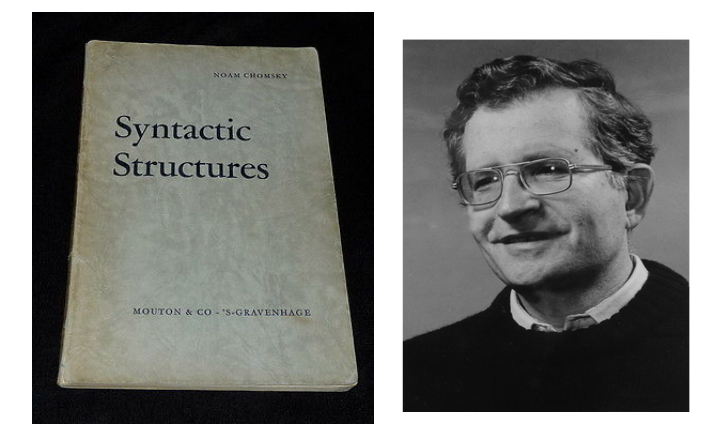
\includegraphics[width=0.9\textwidth]{pics/chomsky.png}\\
        \vspace{0.2cm}
        \scriptsize{\textit{Noam Chomsky}}
      \end{center}
    \end{column}
    \begin{column}{0.6\textwidth}
      \begin{itemize}
        \item Lingüista, filósofo y científico cognitivo estadounidense.
        \item A partir de los 50-60, revoluciona la lingüística con su teoría generativa.
      \end{itemize}
      \textbf{Ideas fundamentales}
      \begin{itemize}
        \item \textbf{Gramática Universal:} principios innatos comunes a todas las lenguas.
        \item \textbf{Dispositivo de adquisición del lenguaje}: Mecanismo biológico.
      \end{itemize}
    \end{column}
  \end{columns}
\end{frame}

% 13. Gramática Universal
\begin{frame}{¿Qué implica la Gramática Universal?}
  \begin{itemize}
    \item Los niños \textbf{no} aprenden el lenguaje solamente de la experiencia; existen estructuras innatas.
    \item Explica la \textbf{rapidez} y \textbf{consistencia} en la adquisición de la lengua materna.
    \item \textbf{Debates actuales:}
      \begin{itemize}
        \item ¿Cuál es el papel de la \textit{cultura} y la \textit{experiencia}?
        \item ¿Se pueden probar empíricamente estos principios innatos?
      \end{itemize}
  \end{itemize}

  \begin{block}{Pregunta}
    \textit{¿Hasta qué punto la “universalidad” puede reflejarse en modelos de NLP que aprenden de datos masivos?}
  \end{block}
\end{frame}

% 14. Michael Tomasello
\begin{frame}{Michael Tomasello (1950- )}
  \begin{columns}
    \begin{column}{0.4\textwidth}
      \begin{center}
        \includegraphics[width=0.9\textwidth]{pics/tomasello.png}\\
        \vspace{0.2cm}
        \scriptsize{\textit{Michael Tomasello}}
      \end{center}
    \end{column}
    \begin{column}{0.6\textwidth}
      \textbf{¿Quién es Tomasello?}
      \begin{itemize}
        \item Psicólogo y antropólogo evolutivo.
        \item Director en el Max Planck Institute for Evolutionary Anthropology.
      \end{itemize}
      \textbf{Propuesta central}
      \begin{itemize}
        \item El lenguaje se construye \textbf{a partir de la interacción social}.
        \item \textbf{Teoría de la mente} y \textbf{capacidad de cooperación} en humanos.
      \end{itemize}
    \end{column}
  \end{columns}
\end{frame}

% 15. Lenguaje como herramienta cultural
\begin{frame}{Tomasello: el lenguaje se moldea en comunidad}
  \begin{itemize}
    \item \textbf{Uso y función pragmática}: Primero surge la comunicación intencional, luego se consolida la forma lingüística.
    \item Enfatiza la \textbf{imitación} y la \textbf{colaboración} en el desarrollo lingüístico de los niños.
    \item \textbf{Comparación con Chomsky:}
      \begin{itemize}
        \item Enfoque en la \textbf{aprendizaje emergente} vs. teoría de un sistema innato.
        \item Insistencia en la influencia social y cultural.
      \end{itemize}
  \end{itemize}

  \vspace{5pt}
  \textbf{Pregunta final:} ¿Puede la interacción social sustituir completamente la necesidad de mecanismos innatos?
\end{frame}

% -------------------------------------------------------------------
%   SECCIÓN: REPRESENTACIÓN DEL LENGUAJE
% -------------------------------------------------------------------
\section{Representación del lenguaje: enfoques}

% 16. ¿Cómo representar el lenguaje computacionalmente?
\begin{frame}{El reto de la representación}
  \begin{block}{Pregunta inicial}
    ¿Qué es el lenguaje a los ojos de un computador? ¿Y el “significado”?
  \end{block}
  \begin{itemize}
    \item \textbf{Múltiples niveles a nivel lingüístico}.
    \item Fonético y fonológico (sonidos)
    \item Morfológico (nivel interno de las palabras)
    \item Sintáctico (nivel de la estructura de las oraciones)
    \item Semántico (nivel de significado)
    \item Pragmático y discursivo (a nivel de uso en contexto)
  \end{itemize}
  \end{frame}

% -------------------------------------------------------------------
%   SECCIÓN: REFLEXIÓN FINAL
% -------------------------------------------------------------------
\section{Reflexión final}

% 18. Reflexión
\begin{frame}{Reflexiones finales}
  \begin{itemize}
    \item El lenguaje \textbf{es más} que un conjunto de palabras y reglas.
    \item \textbf{Dicotomías}: 
      \begin{itemize}
        \item \textit{Individual vs. social}
        \item \textit{Sincronía vs. diacronía}
        \item \textit{Arbitrariedad del significado y significante}
      \end{itemize}
    \item \textbf{Debates}: 
      \begin{itemize}
        \item Innatismo vs. interacción cultural.
        \item Origen del lenguaje y su evolución.
      \end{itemize}
  \end{itemize}
\end{frame}

% 19. Preguntas abiertas
\begin{frame}{Preguntas abiertas para la computación}
  \begin{itemize}
    \item ¿Sigue siendo relevante la lingüística tradicional para la computación en la era de las redes neuronales y los LLM?
    \item ¿Pueden los conceptos de la lingüística enriquecer los estudios computacionales del lenguaje?
    \item ¿Puede la computación ayudar a responder las preguntas abiertas en la lingüística?
\end{itemize}

  \vspace{8pt}
  \textit{La invitación es a seguir buscando respuestas y cuestionando nuestras suposiciones sobre el lenguaje.}
\end{frame}


% -------------------------------------------------------------------
%   DIAPOSITIVA: Lectura obligatoria
% -------------------------------------------------------------------
\begin{frame}{Lectura obligatoria}
  \begin{itemize}
    \item Debes elegir una lectura:
      \begin{enumerate}
        \item Darío Rojas (2015). ¿Por qué los chilenos hablamos como hablamos?
        \item María Victoria Escandell (2011). La semántica. En Invitación a la Lingüística.
        \item Noam Chomsky (1989). El conocimiento del lenguaje, su naturaleza, origen y uso.
      \end{enumerate}
  \end{itemize}
\end{frame}

% -------------------------------------------------------------------
%   BIBLIOGRAFÍA
% -------------------------------------------------------------------
\begin{frame}{Referencias}
  \footnotesize
  \begin{thebibliography}{10}
    \bibitem{saussure1916} Saussure, F. (1916). \textit{Cours de linguistique générale}. Payot.
    \bibitem{chomsky1965} Chomsky, N. (1965). \textit{Aspects of the Theory of Syntax}. MIT Press.
    \bibitem{jakobson1960} Jakobson, R. (1960). \textit{Linguistics and Poetics}. In T. Sebeok (Ed.), \textit{Style In Language}. MIT Press.
    \bibitem{tomasello2003} Tomasello, M. (2003). \textit{Constructing a Language: A Usage-Based Theory of Language Acquisition}. Harvard University Press.
    \bibitem{kohler1929} Köhler, W. (1929). \textit{Gestalt Psychology}. Liveright.
    \bibitem{mikolov2013} Mikolov, T., Chen, K., Corrado, G., \& Dean, J. (2013). \textit{Efficient Estimation of Word Representations in Vector Space}. arXiv preprint arXiv:1301.3781.
  \end{thebibliography}
\end{frame}

\end{document}
